\chapter{Introduction} \label{ch:introduction}

Recent commercial interest in molten salt reactors (MSRs) creates the need for a deep understanding of fission product behavior. Some of the major features that make MSRs so appealing include simplified; fuel cycle, fuel handling, and waste disposal, as well as other versatility and economic benefits \cite{williams1996}. Historically, the only molten salt reactor to ever operate at power was the molten salt reactor experiment experiment (MSRE), an 8-MW(th) nuclear reactor that was operated at the Oak Ridge Nation Laboratory (ORNL) from 1965-1969. The goal of the MSRE was to demonstrate the technical validity of such a reactor at a time when the global supply of uranium was still unknown. This reactor was successfully operated using both ${}^{235}U$ and ${}^{233}U$ \cite{engel1970}. Throughout history, many attempts have been made in order to model the physical and chemical behavior of MSRs. These include many historical reports from the MSRE days on chemistry \cite{grimes1970}, \cite{baes1965}, \cite{cantor1968}, nuclear interactions \cite{nestor1960}, \cite{bell1970}, \cite{prince1962} and mass transport \cite{engel1971}, \cite{peebles1968}, \cite{kedl1967}, \cite{kedl1972}, to name a few. There have also been more recent reports on each of these subjects in the following references: \cite{cammi2011}, \cite{benes2008}, \cite{eades2016}, \cite{wu2017} and \cite{zack2018}. Many of these reports discuss either theory or application in a modeling and simulation framework. The purpose of this thesis is to present a fundamental background on chemical species transport, fission product behavior for a liquid fueled system and implementation of species transport into the Virtual Environment for Reactor Analysis (VERA) for its extension to MSRs (VERA-MSR). Implementation of the generalized species transport solver was accomplished by Dr. Robert Salko and tested by both the author and Dr. Salko \cite{zack2018}. In addition to the generalized species transport, a new multi-phase gas sparging model has been implemented by the author for the analysis of fission product gas removal. 



\section{Nuclear Energy}
Commercial nuclear reactors work on the basis of sustained fission reactions. Nuclear fission is the process whereby an atomic nucleus is split into smaller fragments by the capture of a neutron. These smaller fragments are known as fission products (FPs). The combined mass of the smaller fragments is less than the mass of the original nucleus, and so the missing mass, or "mass defect," is converted into energy using Einstein's famous Equation \ref{eq:Einstein}

\begin{equation}
    \Delta E = \Delta m C^{2}
    \label{eq:Einstein}
\end{equation}

Commercial reactors primarily work with uranium, within which the ${}^{235}U$ isotope is fissile. However, elements such as plutonium and thorium have also been used in power reactors. For ${}^{235}U$ a neutron induced fission reaction is shown in Equation \ref{eq:nuclearFission} \cite{duderstadt1976}.

\begin{equation}
    {}^{235}_{92}U + {}^{1}_{0}n \rightarrow {}^{236}_{92}U^{*} \rightarrow \text{Fission products} + \text{neutrons} + \text{energy}
    \label{eq:nuclearFission}
\end{equation}

About 200 MeV of energy is released from each fission event along with typically two fission fragments and approximately two or three neutrons. Energy release from fission is characterized by the following contributions \cite{fissionBasics}:

\begin{itemize}[label={}]
    \item Kinetic energy of fission products $\approx$ 165 MeV (83\%) 
    \item Gamma rays $\approx$ 7 MeV (4\%)
    \item Kinetic energy of the neutrons $\approx$ 6 MeV (3\%) 
    \item Energy from fission product beta-decay $\approx$ 7 MeV (4\%) 
    \item Gamma rays from fission products $\approx$ 6 MeV (3\%)
    \item Neutrinos from fission products $\approx$ 9 MeV (5\%) 
\end{itemize}

Once fission reactions and neutron populations reach a steady state at a target power level, they are maintained at a constant level so that the rate of fission events and neutrons in a previous generation equal those in the next generation, which characterizes a self-sustaining chain reaction and a "critical" system. If the rate of neutrons generated from the previous generations is increasing, the reaction is said to be "supercritical." Alternatively, if this rate is decreasing, the reaction is said to be "subcritical." Controlling the neutron balance in nuclear reactors is done by balancing the production of neutrons from fission and neutron-producing FPs against the losses due to leakage and absorption of neutrons. Absorbing materials can be removable, such as control blades, or static such as burnable absorbers that are fabricated into the fuel elements, or reactor structural materials.  Leakage is controlled by the geometrical arrangement of fuel and moderating materials and is related to the curvature or gradients of the neutron flux distribution, whereby larger reactors generally have flatter power distributions and lower leakage than smaller reactors.  Neutrons born from fission, approximately 2 to 3 from each fission, can have a wide range of energy values, although they're preferentially born at about 1 to 2 MeV.  In U-235 fueled reactors, neutrons of lower energy have a higher probability of inducing fission, therefore, neutron moderators are commonly employed to slow down the neutrons to thermal energies (below 1 eV), thus allowing more fission events to occur.  The rate at which fission events occur will be discussed later in the manuscript.  

\section{Molten Salt Reactors}
MSRs have two common designs; one in which fissile material held in place like traditional nuclear reactors. In this design, the molten salt simply acts as a heat transfer fluid, carrying the heat away from the fuel elements. The other and more popular design dissolves the fissile material into the circulating salt, thus allowing for fission products to disperse around the primary loop.  This greatly differs from traditional light water reactors (LWRs) where fissile material is maintained in a fixed solid form. Fissile material in MSRs is dissolved in either a chloride or fluoride based salt and is often referred to as the solvent or carrier salt. Fluoride salts are generally used in applications where the reactor operates with neutrons preferentially in the thermal energy spectrum, whereby chloride salts favor the fast energy range.

MSRs produce the unique challenge of allowing fission products to flow throughout the system. Fission products exist in multiple phases (gas, liquid, solid) with each phase interacting with various process equipment contained in the flow loop \cite{grimes1975}. In order to accurately model a dynamic and steady-state fission product behavior, all three phase fields must be resolved.  

This report focuses on three general categories of fission products:

\begin{itemize}
	\item Salt seekers
	\item Noble metals
	\item Noble gases
\end{itemize}

Salt seekers are fission products that will form stable ionic compounds with the carrier salt of interest (XF,XCl) where X is the fission products. Noble metals are fission products which will undergo redox reactions in solution to form solid elemental metals which can plate out in the system. Noble gases are fission products which will be in the gaseous state which are slightly soluble in the carrier salt. These FPs will be processed in an off-gas system \cite{grimes1975}.  

Volatile fission products are a subclass of fission products that can include fission products from both noble metals and gases. These are known as volatile because they do not form stable ionic compounds with the carrier salt. This class of FPs have a noticeable impact on system behavior and cannot be ignored. These impacts include but not limited to: depositing on process equipment, affecting neutron economy, forming collides and other undesired compounds. 


\subsection{Molten Salt Reactor Experiment}
The MSRE was an experiment conducted in the 1960s at ORNL to deduce the validity of molten salt reactors. This was a fluid fueled 8-MW thermal nuclear reactor. During operation, molten salt is continuously circulated about a primary loop containing: the reactor vessel, fuel pump, and heat exchanger. This primary loop contained molten salt with the composition described in Table \ref{tab:MSRE_salt} \cite{engel1970} and a depiction of the process flow diagram is shown in Figure \ref{fig:MSRE_flow_diagram}. 


Salt enters the reactor vessel through orifices at the top portion of the reactor. The holes impart a spiraling flow which moves down the sides of the reactor and up through the bottom head. Salt then flows up the moderator channel tubes shown in Figure \ref{fig:MSRE_fuel_chan}. While the fuel salt is flowing up the channels, graphite moderates the neutrons, inducing fission and power generation. Upon exiting the core, the molten salt then enters the pump bowl shown in Figure \ref{fig:MSRE_pump}. 

Salt enters the fuel pump via the suction port at the bottom of the pump. The pump bowl had two main functions, sample collection and off noble gas removal. The pump bowl had a head space which was constantly purged using a cover gas. Upon discharge, a portion of salt was redirected back into the head space of the pump bowl. This salt was forced through a perforated ring which allowed gas to be removed from the salt via the cover gas. After discharge, the salt flows through a heat exchanger which exits back into the reactor vessel and the process is repeated \cite{engel1970}.

\vspace{12.7mm} %5mm vertical space

\begin{table}[htbp!]
   \caption{\label{tab:MSRE_salt} MSRE operation materials}
   \centering
   \begin{tabular}{l llllllllll}
   \hline
   Fuel Salt & ${}^{7}LiF$-$BeF_{2}$-$ZrF_{4}$-$UF_{4}$ (65.0-29.1-5.0-0.9 mole\%) \\ [1ex]
   Coolant Salt & ${}^{7}LiF$-$BeF_{2}$ (66-34 mole\%) \\ [1ex]
   Moderator & Grade CGB graphite \\ [1ex]
   Salt Containers & Hastelloy-N (68-Ni, 17-Mo, 7-Cr, 5-Fe weight \%) \\ [1ex]
   Cover Gas & Helium/Argon \\ [1ex]
   \hline
   \end{tabular}
\end{table}

\newpage

\vspace{12.7mm} %5mm vertical space

\begin{figure}[p]
  \centering
  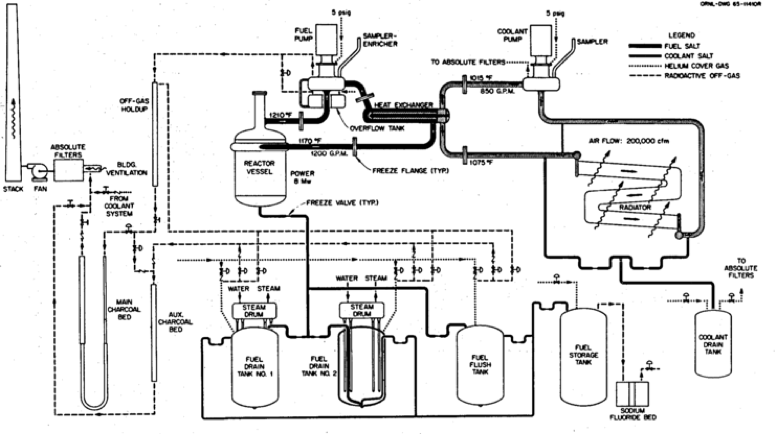
\includegraphics[width=5in]{images/MSRE_flow_diagram.png}\\
  \caption{MSRE process flow diagram}
  \label{fig:MSRE_flow_diagram}
\end{figure} 

\newpage

\begin{figure}[p]
  \centering
  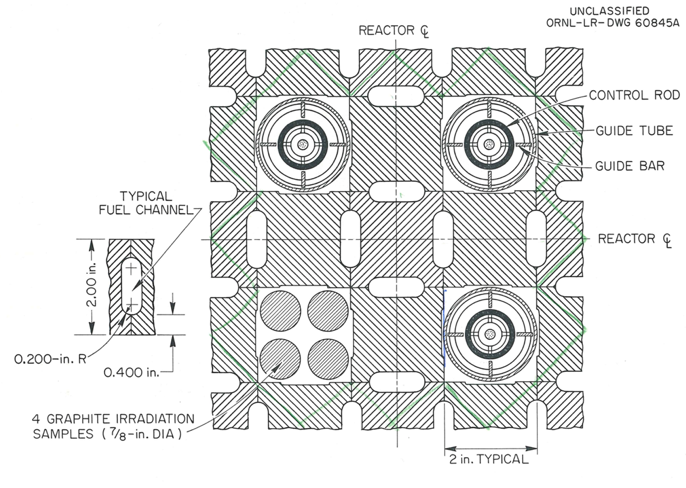
\includegraphics[width=4in]{images/MSRE_fuel_channel.png}\\
  \caption{MSRE graphite fuel channels}
  \label{fig:MSRE_fuel_chan}
\end{figure} 

\vspace{12.7mm} %5mm vertical space

\begin{figure}[p]
  \centering
  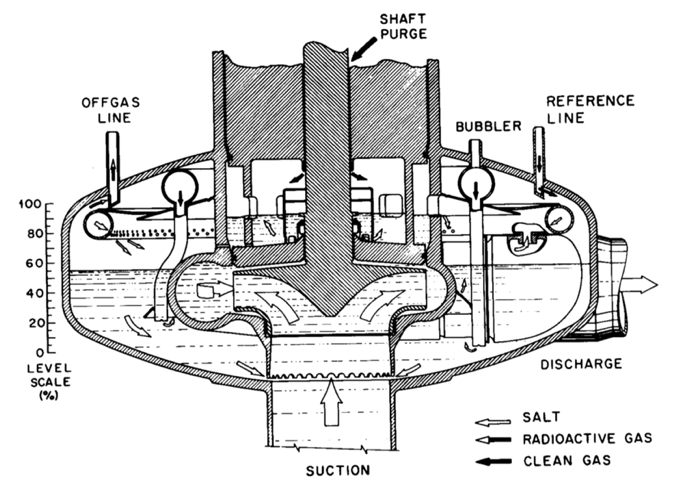
\includegraphics[width=4in]{images/MSRE_pump.png}\\
  \caption{MSRE pump}
  \label{fig:MSRE_pump}
\end{figure} 

\FloatBarrier
\newpage

% Fission produdcts
\subsection{Fission Product Elements}
Although it is possible to generate most of the elements on the Periodic Table, this report will only focus on a portion of fission products which are known to be volatile. Table \ref{tab:common_fission_products} shows common fission products in their respective categories based on MSRE experience \cite{grimes1975}. Elements that have been removed in previous simulation efforts are listed in Table \ref{tab:common_fission_products_removed} \cite{powers2016}. A visual representation of elemental grouping on the periodic table is shown in Figure \ref{fig:periodic_table_fp}. In general, the nuclear reaction for a given fissionable isotope show in equation

% fission equation
\begin{align}
	\ YX_{4} + n  \rightarrow 2FP + 4X^{-}  + \text{neutrons} + \text{energy}
	& \label{eq:fission_reaction}
\end{align}

Where Y is the fissionable isotope, X is the salt of interest (Cl or F) and FP are the fission products produced.

\subsubsection{Salt Seekers}
Salt seekers form stable fluoride or chloride compounds which are soluble in the carrier salt. These compounds are almost completely found in the molten fuel \cite{grimes1970}. Stability of salt seekers is approximated by energy of formation. Compounds that have a more negative energy of formation will be more stable than those same elements forming other compounds with higher heats of formation. Many of the salt seeker fission products are rare earth elements with high neutron capture cross sections \cite{baes1974}. Neutron economy can be increased if these elements are separated from the reaction medium.  

\subsubsection{Noble Metals}
Noble metals are born as ions from fission and decay of their precursors. They are unstable in the fuel salt and do not live as ions for very long. Once they are born they quickly undergo reduction reactions and are homogeneously dispersed in the salt. This group of fission products tend to deposit on surfaces inside the flow loop, which can include: heat exchanger, pipes, reactor vessel and moderator. Noble metals also deposit on liquid-gas interfaces such as bubble surfaces and display some properties of surface active agents \cite{kedl1972}. 

\newpage

% Table of common fission products
\begin{table}[p]
   \caption{\label{tab:common_fission_products} Common fission products}
   \centering
   \begin{threeparttable}
   \begin{tabular}{l llllllllll}
   \hline
   \textbf{Group} & \textbf{Element}\\
   \hline 
   Salt seekers & Rb, Sc, Sr, Ba, Y, Zr, Lanthanides \\ [1ex]
   Noble metals & $Nb^{a}$, Mo, Tc, Ru, Rh, Pb, Ag, Sb, $Te^{b}$, $I^{b}$ \\ [1ex]
   Noble gases & Xe, Kr \\ [1ex]
   \hline
   \end{tabular}
   \begin{tablenotes}\footnotesize
   \item[a] Niobium is borderline and depends on redox condition of the salt 
   \item[b] Iodine can form iodides and remain in the slat however it is included because of its tellurium predecessor \cite{grimes1975}
   \end{tablenotes}
   \end{threeparttable}
\end{table}


\vspace{12.7mm} %5mm vertical space

% table of fissions products that people want to remove
\begin{table}[p]
   \caption{\label{tab:common_fission_products_removed} Common fission products removed from salt}
   \centering
   \begin{tabular}{l llllllllll}
   \hline
   \textbf{Group} & \textbf{Element}\\
   \hline 
   Volatile gases & Xe, Kr \\ [1ex]
   Noble metals & Se, Nb, Mo, Tc, Ru, Rh, Pb, Ag, Sb, Te \\ [1ex]
   Seminoble metals & Zr, Cd, In, Sn \\ [1ex]
   Volatile fluorides & Br, I \\ [1ex]
   Rate earth elements & Y, La, Ce, Pr, Nd, Pm, Sm, Gd, Eu \\ [1ex]
   Discard & Rb, Sr, Cs, Ba \\ [1ex]
   \hline
   \end{tabular}
\end{table}

\FloatBarrier

\newpage

% periodic table figure. Need to find source for actual table picture. Or find a new picture and redo the coloring
\begin{figure}[p]
  \centering
  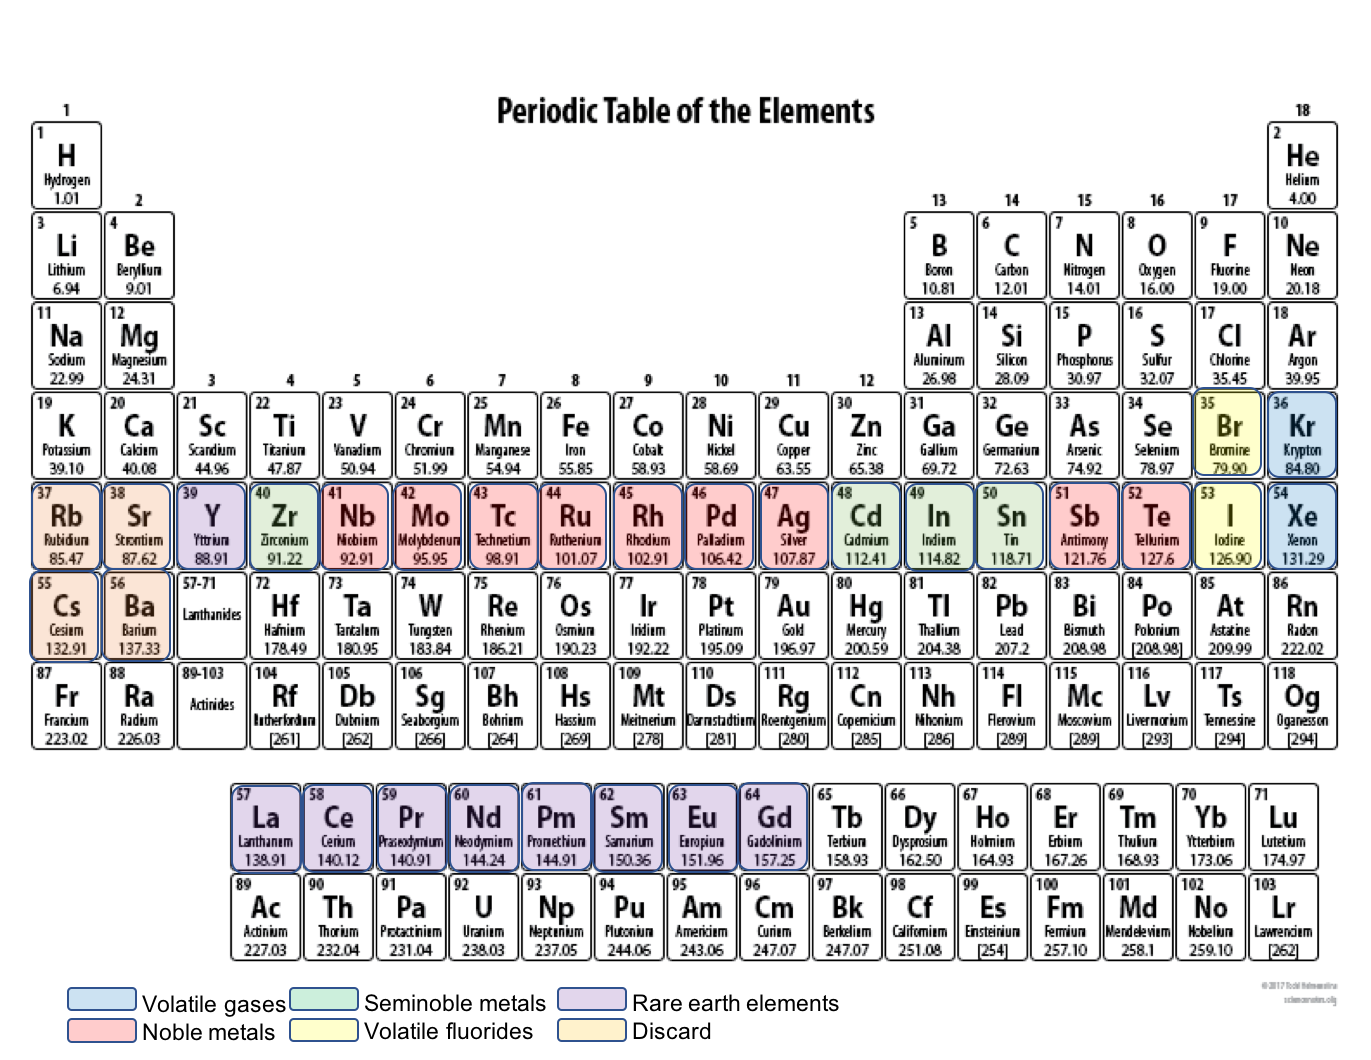
\includegraphics[width=6in]{periodic_table.png}\\
  \caption{Periodic table with highlighted fission products.}
  \label{fig:periodic_table_fp}
\end{figure} 

\FloatBarrier
\newpage

\subsubsection{Noble Gases}
Fission product noble gases Xe and Kr form no compounds in a MSR and are sparingly soluble in the carrier salt. Because of this, these noble gases tend to collect in any circulating voids contained in the flow loop. Many present and past MSR designs utilize this fact and include gas stripping processes which entrained bubbles in the carrier salt. Process equipment may also be permeable to fission product gases. In the case of the MSRE, moderator graphite was permeable and influences steady-state and transient noble gas behavior \cite{grimes1970}. Xenon is of particular interest due to its isotope ${}^{135}$Xe which has a neutron absorption cross section many orders of magnitude higher than the fissile material dissolved in the fuel. Xenon robs the reactor of neutrons and will eventually shut down the reactor if not properly handled. 

\section{VERA}
The Consortium for Advanced Simulation of Light Water Reactors (CASL) is the US Department of Energy's (DOE) first Energy Innovation Hub, a large collaboration among nuclear engineering research institutions and commercial partners around the globe, headquartered at ORNL. CASL's mission is to confidently predict the performance of existing and the next generation of advanced nuclear reactors \cite{casl}. In doing so, they have developed the Virtual Environment of Reactor Applications Core Simulator (VERA-CS), a collection of software tools utilized for modeling LWRs. VERA performs coupled multi-physics simulations involving reactor nuclear physics, thermal-hydraulics, LWR chemistry, isotopic depletion and fuel performance. In order to handle the industry's growing interest in advanced nuclear reactors, VERA-MSR is currently under development to extends its capabilities to model MSRs. In addition to the physics packages already supported in VERA, two more needed to be added, these include species transport and thermochemical state, as shown in Figure \ref{fig:multiphysicsMSR}.

 
For thermal-hydraulic calculations VERA uses CTF, a modernized version of COBRA-TF which was originally developed in the early 1980s by Pacific Northwest Laboratory \cite{zack2018}. CTF uses a two-fluid model broken up into three separate fluid fields: liquid film, liquid droplets and vapor, each with its own set of conservation equations. The governing sets of 9 equations is turned into 8 by assuming that liquid and droplet fields are in thermal equilibrium and share an energy equation. Discretization is done on a 3-D finite volume Cartesian mesh with scalar and momentum cells staggered on top of one another. The governing set of equations are formatted either using the full 3-D solution or using a sub-channel approach and are solved using the SIMPLE method \cite{salko2017}. After a CTF solves its governing set of mass, momentum and energy equations, temperature, pressure and the velocity fields are known, these values are then utilized in species transport. Temperature and pressure fields are required for two-phase interfacial area calculations. The fluid velocity field is used in the convection flux contribution for species transport.  

\vspace{12.7mm} %5mm vertical space

\begin{figure}[h]
  \centering
  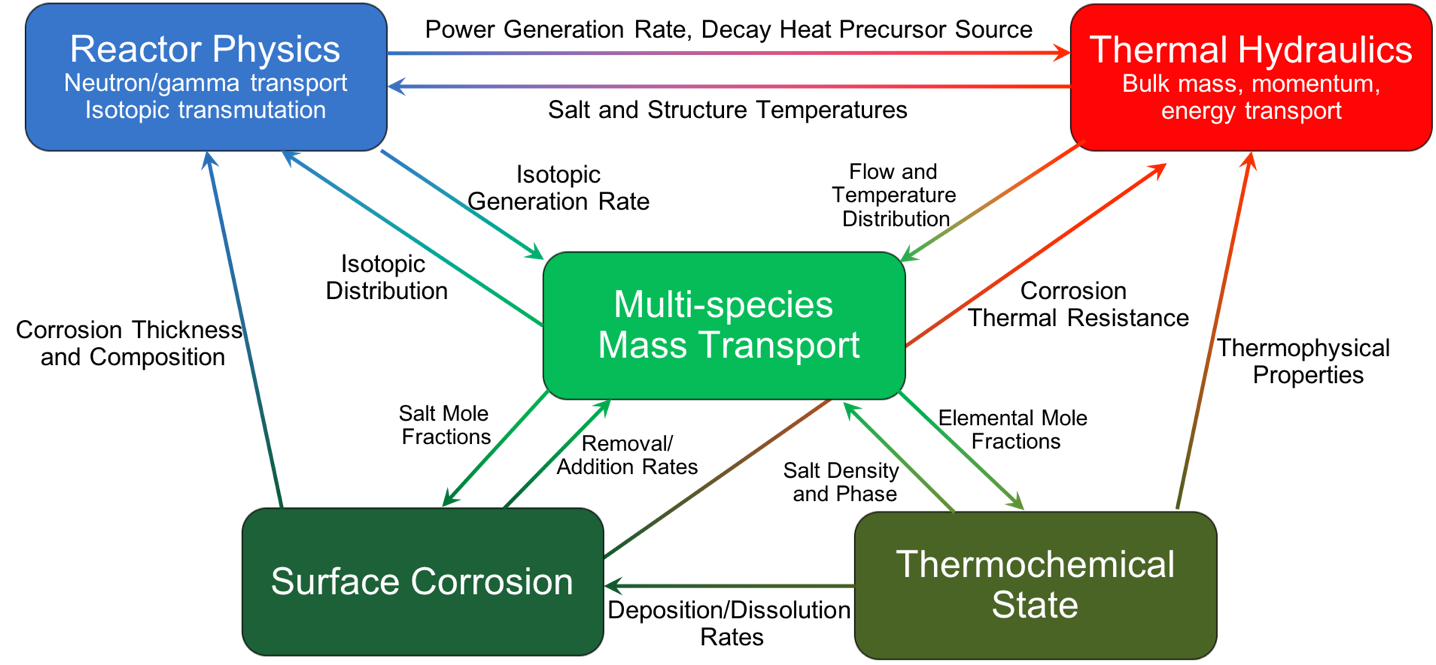
\includegraphics[width=6in]{images/multiphysics.png}\\
  \caption{Multi-physics simulations need for MSRs}
  \label{fig:multiphysicsMSR}
\end{figure}